\documentclass{beamer}
\usepackage[utf8]{inputenc}
\usepackage[notocbib]{apacite}
\usepackage{graphicx, amsmath, algorithm, tikz, algpseudocode, subcaption}%, algcompatible}% algorithmic}
\usepackage{hyperref}

\usetheme{Warsaw}
\usefonttheme{professionalfonts,serif,structuresmallcapsserif}

\setbeamertemplate{footline}
{
  \leavevmode%
  \hbox{%
  \begin{beamercolorbox}[wd=.333333\paperwidth,ht=2.25ex,dp=1ex,center]{author in head/foot}%
    \centering
    \insertauthor
  \end{beamercolorbox}%
  \begin{beamercolorbox}[wd=.555555\paperwidth,ht=2.25ex,dp=1ex,center]{title in head/foot}%
    \centering
    \insertsubtitle
  \end{beamercolorbox}%
  \begin{beamercolorbox}[wd=.1111111\paperwidth,ht=2.25ex,dp=1ex,right]{date in head/foot}%
    \centering
    \insertframenumber{} / \inserttotalframenumber%\hspace*{2em} 
  \end{beamercolorbox}}%
  \vskip0pt%
}
 
%Information to be included in the title page:
\title{Wildfire Spreading Model using a Parallel Implementation of Cellular Automata}
\subtitle{Advanced Applied Parallel Programming}
\author{Daniel San Martín}
\institute{Departamento de Informática \\ Universidad Técnica Federico Santa María}
\date{March 2018}
 
\usebackgroundtemplate{
  \tikz[overlay,remember picture] 
  \node[opacity=0.3, at=(current page.south east), anchor=south east, yshift=20pt, xshift=-10pt, inner sep=0pt] {
    
\includegraphics[width=0.15\textwidth]{figures/usm.jpg}};
}

\AtBeginSection[]
{
  \begin{frame}
    \frametitle{Outline}
    \tableofcontents[currentsection]
  \end{frame}
}

\begin{document}
 
  \frame{\titlepage}

  \begin{frame}{Outline}
    \tableofcontents
  \end{frame}

  \section{Introduction}

      \begin{frame}{Introduction}
        \begin{itemize}
          \item<1-> Wildfires are one of the most harmful phenomena in Chile.
          \item<2-> Fires may start by varied reasons, ranging from reckless human behavior to extreme weather 
              and environmental conditions.          
        \end{itemize}
        \begin{figure}
          \centering
          \includegraphics<3->[width=0.5\textwidth]{figures/wildfire.jpg}
          \label{fig:wildfire}
        \end{figure}
      \end{frame}

      \begin{frame}{Introduction}
        \begin{itemize}
          \item<1-> Around $50000$ hectares are burnt yearly, and in certain occasions up to $100000$ 
              hectares \cite{fireCONAF}.
          \item<2-> Fire spreading dynamics has gathered large attention from the scientific community.
          \item<3-> Wildfires are modelled using continuous or discrete models, or a combination of both.
        \end{itemize}
          \begin{figure}
          \centering
          \begin{subfigure}{.5\textwidth}
            \centering
            \includegraphics<4->[width=.6\linewidth]{figures/model-1.jpg}
          \end{subfigure}%
          \begin{subfigure}{.5\textwidth}
            \centering
            \includegraphics<4->[width=.5\linewidth]{figures/model-2.jpg}
          \end{subfigure}
        \end{figure}
      \end{frame}

   
  \section{Problem}    
    \subsection{Formalization}
      
      \begin{frame}{Formalization}
        \begin{block}{Problem}
          Build a suitable model to be incorporated into a video-game-based 
          simulator to allow assessment of decision making during wildfire combat 
          involving different agencies which are part of the response system in Chile.
        \end{block}
      \end{frame}
      
      
    \subsection{Solution}

      \begin{frame}{Solution}
        \begin{itemize}
          \item<1-> The fire model was constructed integrating environmental factors, forest 
            fuel, topography with a discrete model based in Cellular Automata (CA) which interact 
            and evolve in discrete time steps.
          \item<2-> To include the dynamic component, it was necessary to enhance 
            the computation of the model with parallel computing techniques.
        \end{itemize}
      \end{frame}
      
      \begin{frame}{Solution}
        \begin{itemize}
          \item<1-> \textbf{Environmental factors}
            \begin{itemize}
              \item<1-> Wind's speed and direction have a direct effect over fire spreading.
              \item<2-> Temperature has a direct effect over fire spreading.
              \item<3-> Relative humidity has an inversely effect over fire spreading.
              \item<4-> Pressure has an inversely effect over fire spreading.
            \end{itemize}
          \item<5-> \textbf{Forest fuels}: All the vegetation elements, woody or herbaceous, 
            alive or dead that may be flammable.
          \item<6-> \textbf{Topography}: It influences over the two above factors, the fuel and weather,
            modifying or altering them.
        \end{itemize}
      \end{frame}
      
      \begin{frame}{Solution}
        \begin{itemize}
          \item<1-> \textbf{Cellular Automata}
            \begin{itemize}
              \item<2-> Spatial Dimension: We used a 2D spatial dimension based on a grid of size $M\times N$.
                Each cell is located over the grid in positions $(i,j)$.
              \item<3-> Neighborhood: This CA model use the Moore Neighborhood, defined as
                \begin{equation}
                  N_{(i_0,j_0)}^M = \{(i,j): ~ |i-i_0|\leq r, ~ |j-j_0|\leq r \}.
                \end{equation}
                for a cell $(i_0, j_0)$ in a radius $r=1$.
              \item<4-> Cell States: In this work we use $S_{i,j}\in \{0, 1, 2, 3, 4\}$ where nonflammable = $0$; 
                flammable = $1$; burning = $2$; burnt = $3$; extinguished = $4$.
              \item<5-> Transition Function: $F: DW \rightarrow S$ where,
            \end{itemize}
        \end{itemize}
      \end{frame}
      
      \begin{frame}{Solution}
        $DW$ is a discretized world that contains states $S$, temperature $T$, humidity $H$, wind speed $W_s$ 
        and direction $W_d$, fuel $C$ and the probability threshold of change from state $a$ to $b$ $F_{ab}$. 
        All this variables are matrices with values between $0$ to $1$. 
      \end{frame}

      \begin{frame}{Solution}
        \begin{figure}
          \centering
          \resizebox{0.5\textwidth}{!}{
            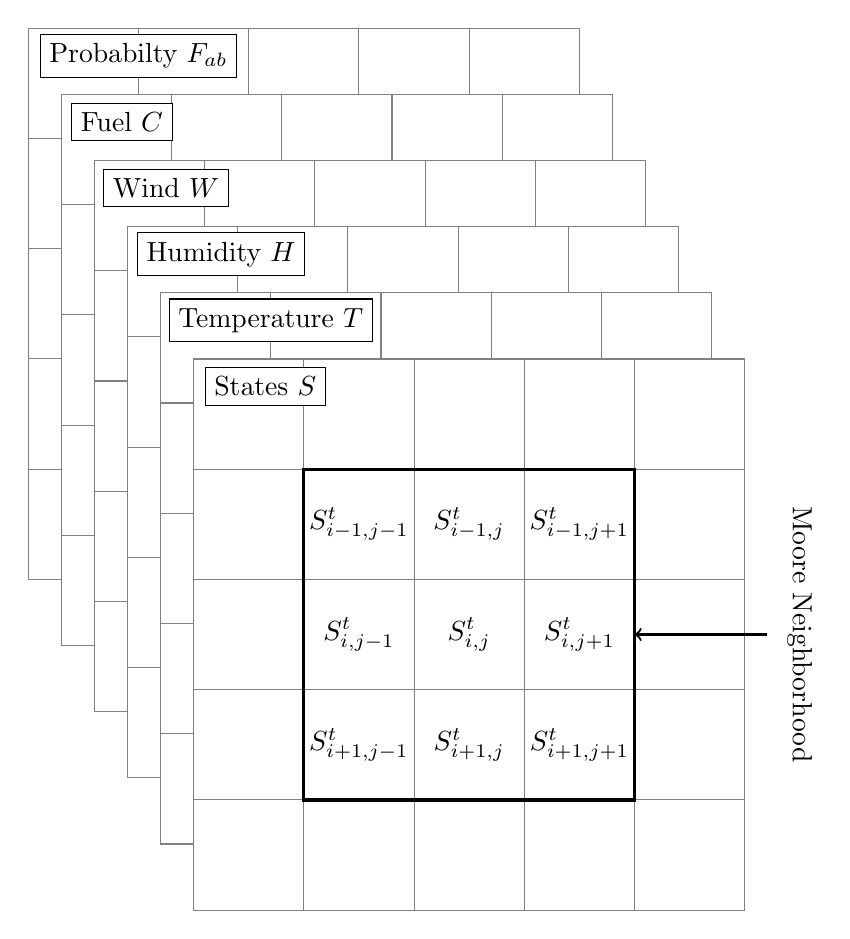
\begin{tikzpicture}[scale=1.4]
    
    \begin{scope}[xshift=-1.5cm, yshift=3cm]
        \draw[draw=gray, fill=white] (0, 0) grid (5, 5) rectangle (0,0); % grid
        \node[draw, fill=white] at (1, 4.75) {Probabilty $F_{ab}$}; % Layer name
    \end{scope}
    
    \begin{scope}[xshift=-1.2cm, yshift=2.4cm]
        \draw[draw=gray, fill=white] (0, 0) grid (5, 5) rectangle (0,0); % grid
        \node[draw, fill=white] at (.55, 4.75) {Fuel $C$}; % Layer name
    \end{scope}

    \begin{scope}[xshift=-.9cm, yshift=1.8cm]
        \draw[draw=gray, fill=white] (0, 0) grid (5, 5) rectangle (0,0); % grid
        \node[draw, fill=white] at (.65, 4.75) {Wind $W$}; % Layer name
    \end{scope}
    
    \begin{scope}[xshift=-.6cm, yshift=1.2cm]
        \draw[draw=gray, fill=white] (0, 0) grid (5, 5) rectangle (0,0); % grid
        \node[draw, fill=white] at (.85, 4.75) {Humidity $H$}; % Layer name
    \end{scope}
    
    \begin{scope}[xshift=-.3cm, yshift=.6cm]
        \draw[draw=gray, fill=white] (0, 0) grid (5, 5) rectangle (0,0); % grid
        \node[draw, fill=white] at (1, 4.75) {Temperature $T$}; % Layer name
    \end{scope}

    \begin{scope}
        \draw[draw=gray, fill=white] (0, 0) grid (5, 5) rectangle (0,0); % grid
        \draw[very thick] (1, 1) rectangle (4,4); % Moore neighborhood
        
        % States
        \node at (2.5, 2.5) {$S_{i,j}^t$};
        \node at (2.5, 3.5) {$S_{i-1,j}^t$};
        \node at (2.5, 1.5) {$S_{i+1,j}^t$};
        \node at (1.5, 2.5) {$S_{i,j-1}^t$};
        \node at (3.5, 2.5) {$S_{i,j+1}^t$};
        \node at (1.5, 3.5) {$S_{i-1,j-1}^t$};
        \node at (1.5, 1.5) {$S_{i+1,j-1}^t$};
        \node at (3.5, 3.5) {$S_{i-1,j+1}^t$};
        \node at (3.5, 1.5) {$S_{i+1,j+1}^t$};
        
        % Layer name
        \node[draw, fill=white] at (.65, 4.75) {States $S$};

        \node [rotate=-90] at (5.5, 2.5) {Moore Neighborhood};
        \draw[->, thick] (5.2, 2.5) -- (4, 2.5);
    \end{scope}
    
\end{tikzpicture}
          }    
          \caption{Discrete World ($DW$).}
          \label{fig:discrete_world}
        \end{figure}
      \end{frame}

      \begin{frame}{Solution}
        Formally, we define the transition as
        \begin{equation}
          S_{i,j}^{t+1} =
          \begin{cases}
            2, & \text{if} ~ S_{i,j}^{t} = 1 ~ \text{and} ~ f_{12} \geq F_{12} \\
            2, & \text{if} ~ S_{i,j}^{t} = 4 ~ \text{and} ~ f_{42} \leq F_{42} \\
            3, & \text{if} ~ S_{i,j}^{t} = 2 ~ \text{and} ~ f_{23} \leq F_{23} \\
            4, & \text{if} ~ S_{i,j}^{t} = 3 ~ \text{and} ~ f_{24} \leq F_{24}
          \end{cases},
          \label{eq:transition_rule}
        \end{equation}
        where functions $f$ are defined by
      \end{frame}
      
      \begin{frame}{Solution}
        \begin{itemize}
          \item Function $f_{12}$:
            \begin{itemize}
              \item The environmental factors $E$:
                \begin{equation}
                  E_{i,j} = \frac{W_{d_{i,j}} ~ C_{i,j} ~ T_{i,j} ~ W_{s_{i,j}}}{H_{i,j} ~ P_{i,j}}.
                \end{equation}
              \item The burning states of neighborhood $p(N_b)$:
                \begin{equation}
                  p(N_b)_{i,j} = \frac{N_b}{8},
                \end{equation}
                where $N_b$ is the number of burning state neighboring cells.
            \end{itemize}
            Then, $f_{12}$ is computed by
            \begin{equation}
              f_{12} = \alpha ~ E_{i,j} + \beta ~ p(N_b)_{i,j}.
            \end{equation}
          \item Functions $f_{23}, f_{24}, f_{42}$ are random values between $0$ and $1$ 
            and $F_{23}, F_{24}, F_{42}$ are threshold parameters.
        \end{itemize}
      \end{frame}            
          
      \begin{frame}{Solution}
        \begin{itemize}
          \item<1-> The development of the algorithm needs to perform a tessellation of the area 
            to be simulated, where each cell represents the state of a square portion of the terrain. 
          \item<2-> The model works with a world discretized by layers ($DW$), where each layer contains 
            the information of the components described before.
        \end{itemize}
      \end{frame}
      
      \begin{frame}{Algorithm}
        \begin{algorithm}[H]
          \begin{algorithmic}
            \State{$S^0 \gets $ Initialize cell's states.}
            \State{$DW \gets $ Initialize discrete world.}
            \For{$t=0$ to $T_{max}$}
                \State{$S^{t+1} \gets spreading(S^t, DW)$}
            \EndFor
          \end{algorithmic}
          \caption{Main Algorithm}
          \label{alg:main}
        \end{algorithm}
      \end{frame}
      
      \begin{frame}{Algorithm}
        \vspace{-0.5cm}
        \begin{algorithm}[H]
          \footnotesize
          \begin{algorithmic}
            \Procedure{spreading}{$S^t, DW$}
              \State{$N \gets$ number of rows in $DW$}
              \For{$i=0$ to $N_{threads}-1$}
                \State{$delta \gets N / N_{threads}$}
                \State{$start \gets i\cdot delta$}
                \If{$i = N_{threads}-1$}
                    \State{$end \gets$ $N$}
                \Else
                    \State{$end \gets (i+1)\cdot delta$}
                \EndIf
                \State{$S \gets subSpreading(start, end, S^t, DW)$}
              \EndFor
              \For{$i=0$ to $N_{threads}-1$}
                \State{Thread's join}
              \EndFor
              \State{\textbf{return} $S$}
            \EndProcedure
          \end{algorithmic}
          \caption{Spreading Algorithm}
          \label{alg:spreading}
        \end{algorithm}
      \end{frame}
      
      \begin{frame}{Algorithm}
        \begin{algorithm}[H]
          \begin{algorithmic}
            \Procedure{subSpreading}{$start, end, S^t, DW$} 
              \State{$N \gets$ number of columns in $DW$.}
              \For{$i=start$ to  $end$}
                \For{$j=0$ to $N$}
                  \State{Compute $S_{i,j}^t$ using equation (\ref{eq:transition_rule}) with $S^t$ and $DW$.}
                \EndFor
              \EndFor
              \State{\textbf{return} $S_{i,j}^t$}
            \EndProcedure
          \end{algorithmic}
          \caption{Sub-spreading Algorithm}
          \label{alg:subspreading}
        \end{algorithm}
      \end{frame}
      
      \begin{frame}{Algorithm}
        \begin{figure}
          \centering
          \resizebox{0.65\textwidth}{!}{
            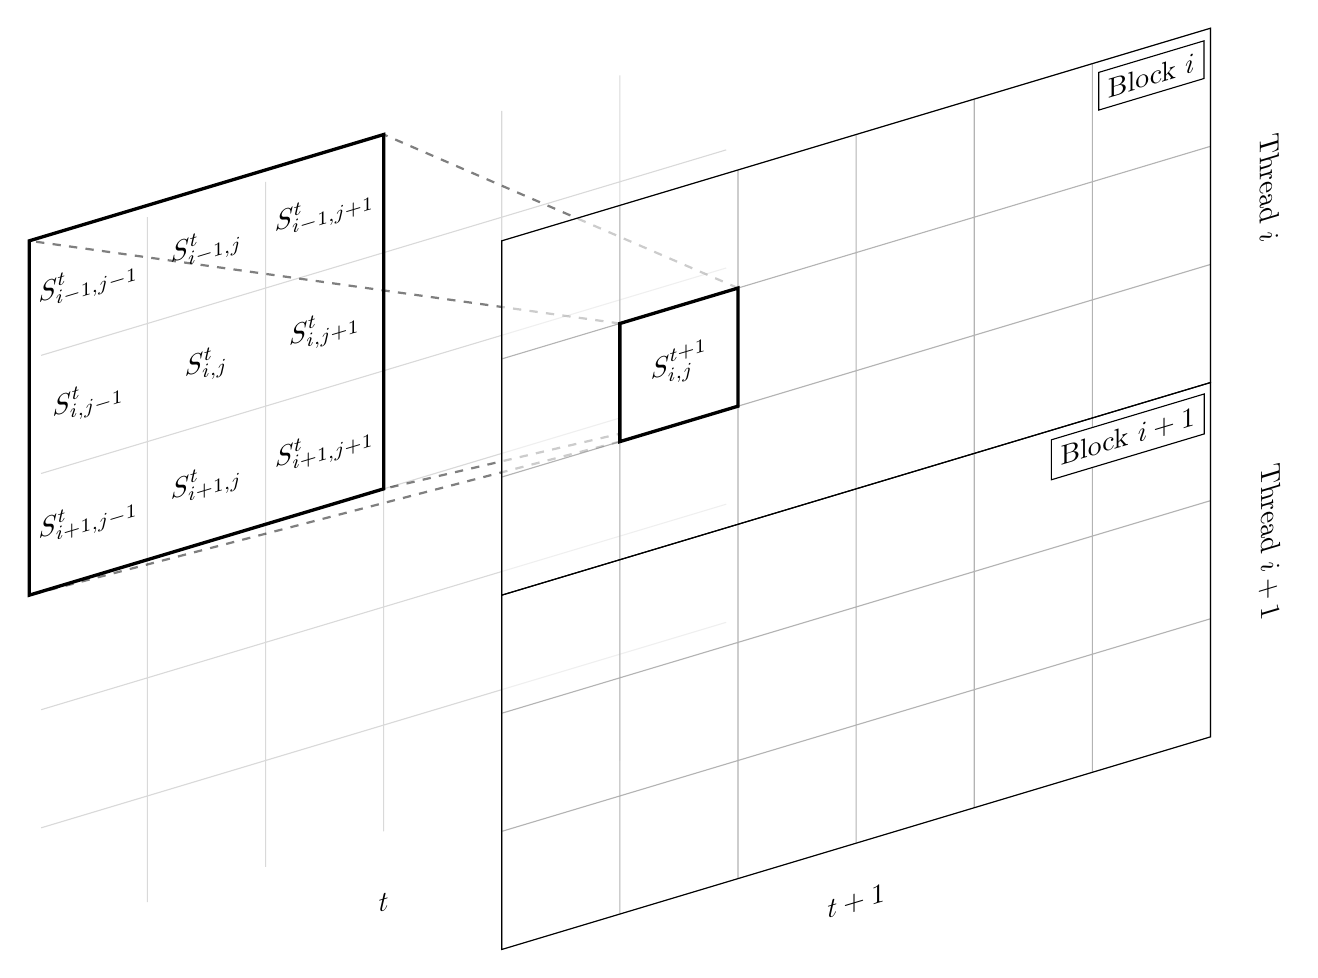
\begin{tikzpicture}[scale=1.5]

     \begin{scope}[every node/.append style={yslant=0.3},yslant=0.3]
        \draw[gray, opacity=0.3] (0.1, 0.1) grid (5.9, 5.9);
        \draw[very thick] (0, 6) -- (3, 6) --  (3, 3) -- (0, 3) -- cycle;
        %\draw[ultra thick] (-1, 3) -- (7,3);
        \node[anchor=center] at (1.5, 4.5) {$S_{i,j}^t$};
        \node[anchor=center] at (1.5, 5.5) {$S_{i-1,j}^t$};
        \node[anchor=center] at (1.5, 3.5) {$S_{i+1,j}^t$};
        \node[anchor=center] at (0.5, 4.5) {$S_{i,j-1}^t$};
        \node[anchor=center] at (2.5, 4.5) {$S_{i,j+1}^t$};
        \node[anchor=center] at (0.5, 5.5) {$S_{i-1,j-1}^t$};
        \node[anchor=center] at (0.5, 3.5) {$S_{i+1,j-1}^t$};
        \node[anchor=center] at (2.5, 5.5) {$S_{i-1,j+1}^t$};
        \node[anchor=center] at (2.5, 3.5) {$S_{i+1,j+1}^t$};
        \node[anchor=center] at (3, -0.5) {$t$};
    \end{scope}
    
    \begin{scope}[xshift=4cm,every node/.append style={yslant=0.3},yslant=0.3]
        \draw[dashed, thick, opacity=0.5] (1, 5) -- (-4, 7.2);
        \draw[dashed, thick, opacity=0.5] (1, 4) -- (-4, 4.2);
        \draw[dashed, thick, opacity=0.5] (2, 5) -- (-1, 7.2);
        \draw[dashed, thick, opacity=0.5] (2, 4) -- (-1, 4.2);
        \draw[draw=gray, fill=white, opacity=0.6] (0, 0) grid (6, 6) rectangle (0, 0);
        \draw[very thick, fill=white] (1, 5) -- (2, 5) --  (2, 4) -- (1, 4) -- cycle;
        
        %\draw[ultra thick] (-1, 3) -- (7,3);
        \node[anchor=center] at (1.5, 4.5) {$S_{i,j}^{t+1}$};
        
        \draw (0,3) rectangle (6,6);
        \draw (0,0) rectangle (6,3);
        
        %\draw[dash dot, ultra thick] (-1, 3) -- (7, 3);
        \node[anchor=center] at (3, -0.5) {$t+1$};
        \node[draw, fill=white] at (5.5, 5.75) {Block $i$};
        \node[draw, fill=white] at (5.3, 2.75) {Block $i+1$};
        \node [rotate=-90] at (6.5, 4.5) {Thread $i$};
        \node [rotate=-90] at (6.5, 1.5) {Thread $i+1$};
    \end{scope}
    
\end{tikzpicture}
          }    
          \caption{\emph{SubSpreading} computing a matrix block.}
          \label{fig:thread}
        \end{figure}
      \end{frame}
      
  \section{Results}
      \subsection{Evaluation}
      
      \begin{frame}{Evaluation}
        \begin{itemize}
          \item<1-> Using a square grid of size $N \times N$ and defining the maximum number
            of discrete times $T_{max}$ we estimate a computational complexity of $O(T_{max}\cdot N^2)$. 
          \item<2-> If we choose $T_{max} << N$ the complexity is about $O(N^2)$, but it 
            may change a lot if $T_{max}\sim N$ increasing the complexity to $O(N^3)$. 
          \item<3-> This is the main  motivation of to include the use of threads in the computing of the model.
        \end{itemize} 
      \end{frame}
      
      \begin{frame}{Evaluation}
        The experiments were made using a fixed $T_{max}=50$, for $1$ to $4$ number of threads, repeating the 
        simulations $10$ times per $N$.
        \begin{table}[!ht]
          \renewcommand{\arraystretch}{1.3}
          \centering
          \caption{Summary of the average times in seconds.}
          \label{tab:results}
          \begin{tabular}{c||rrrr}
            \hline
            Threads & $N=100$ & $N=500$ & $N=1000$ & $N=1500$ \\ \hline\hline
            1       & $0.198$   & $8.023$   & $32.861$   & $72.464$   \\
            2       & $0.135$   & $5.147$   & $19.695$   & $44.407$   \\
            3       & $0.163$   & $4.825$   & $18.852$   & $41.626$   \\
            4       & $0.220$   & $4.650$   & $18.055$   & $41.458$  
          \end{tabular}
        \end{table}
      \end{frame}
      
      \begin{frame}{Evaluation}
        \begin{figure}[!ht]
          \centering
          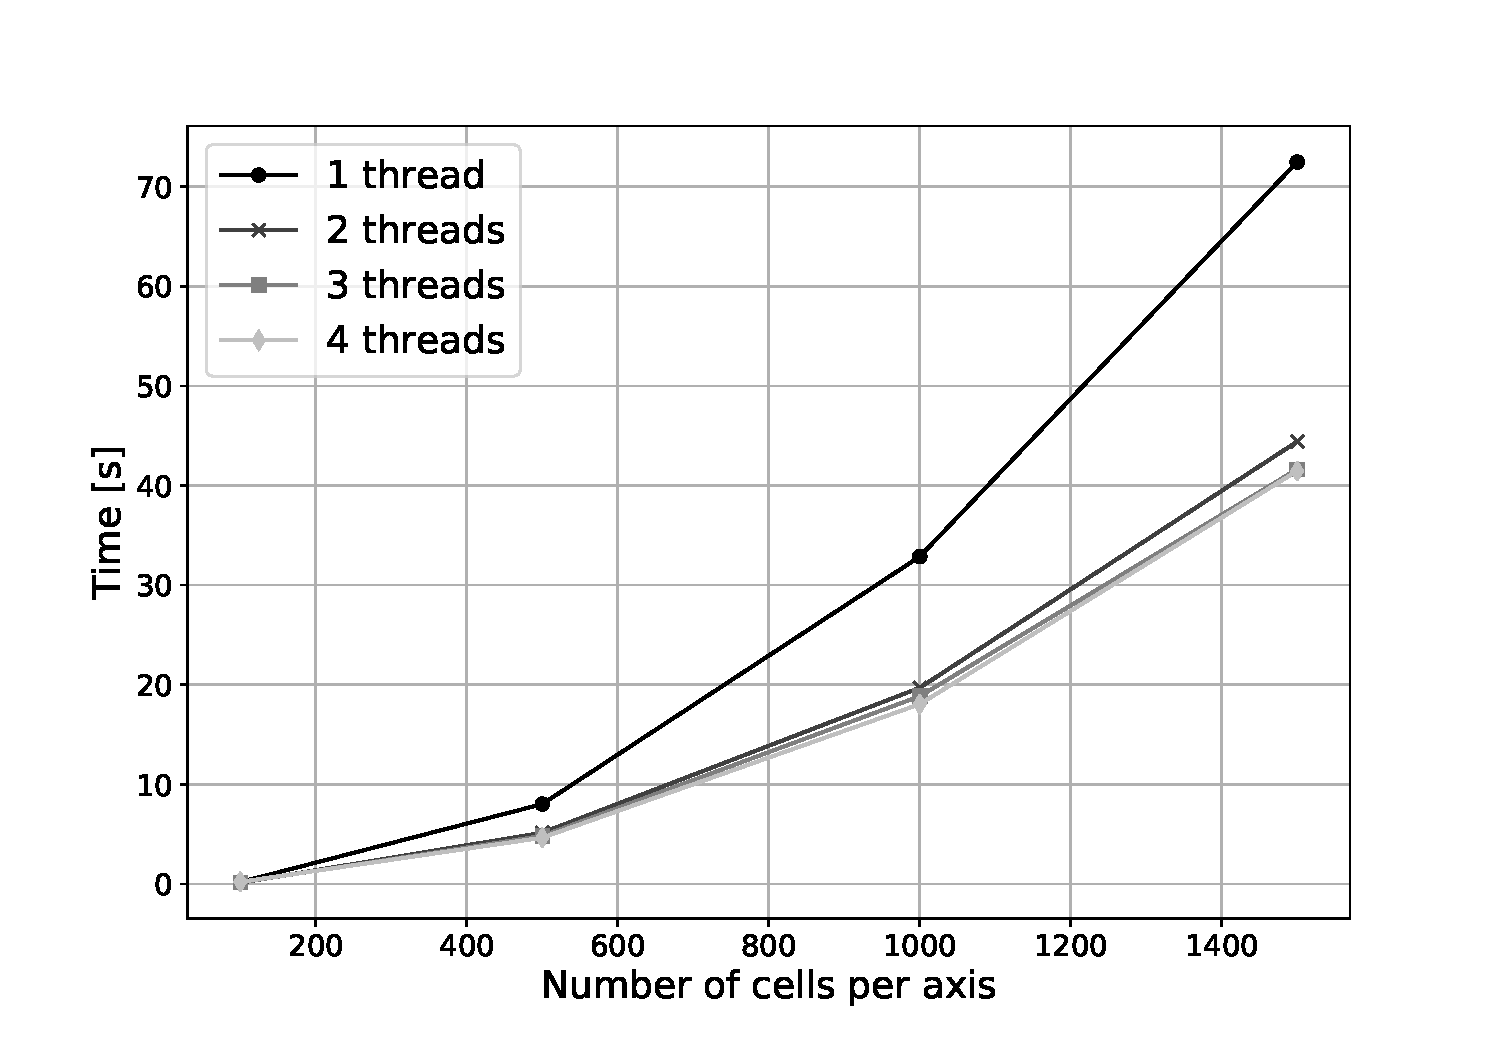
\includegraphics[width=3in,height=3in,clip,keepaspectratio]{figures/benchmark.pdf}
          \caption{Threads' performance comparison.}
          \label{fig:benchmark}
        \end{figure}
      \end{frame}
      
      \begin{frame}{Evaluation}
        \begin{table}[!ht]
        \renewcommand{\arraystretch}{1.3}
        \centering
        \caption{Speedups results.}
        \label{tab:speedups}
        \begin{tabular}{c||rrrr}
          \hline
          Threads & $N=100$ & $N=500$ & $N=1000$ & $N=1500$ \\ \hline\hline
          2       & $1.47$ & $1.56$ & $1.67$ & $1.63$ \\
          3       & $1.21$ & $1.66$ & $1.74$ & $1.74$ \\
          4       & $0.90$ & $1.73$ & $1.82$ & $1.75$  
          \end{tabular}
        \end{table}
      \end{frame}
      
      \begin{frame}{Evaluation}
        \begin{figure}[!ht]
          \centering
          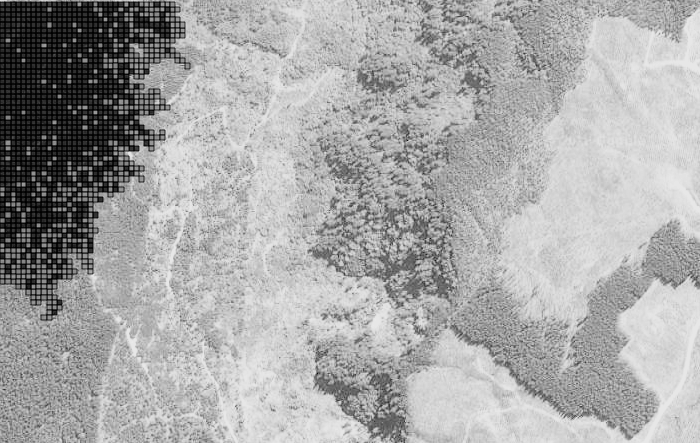
\includegraphics[width=3in,height=3in,clip,keepaspectratio]{figures/simulation_gray.png}
          \caption{piece of map simulated for $N=1500$, $T=30^{\circ}$C, $H=50$\%, 
              $W_s=40$ km/hr, $W_d=90^{\circ}$, $P=50$ hPa, $F_{23} = F_{24}= F_{42} = 0.1$..}
          \label{fig:simulation}
        \end{figure}
      \end{frame}

      \subsection{Validation/Discussion}
        \begin{frame}{Validation/Discussion}
          \begin{itemize}
            \item<1-> There are different fire propagation models, but each one depends on the 
              conditions of each study place.
            \item<2-> The wildfire dynamics generated with the prototypes are consistent with what 
              CONAF has observed in past devastating wildfires occurring in Chile.
            \item<3-> The main problem with wildfire models based on differential equations is the 
              computational cost associated with the resolution of the system of equations.
            \item<4-> The complexity of the models is related to the realism and dynamism they have.
          \end{itemize}
        \end{frame}
      
      \subsection{Conclusion}
        \begin{frame}{Conclusion}
          \begin{itemize}
            \item<1-> The incorporation of parallel techniques allows the model to compute enough 
              states in discrete times to show a qualitatively realistic result for the specialists' requirements.
            \item<2-> The use of multithreads is a good strategy to apply to this problem given 
              the characteristics of the discrete world and the independence of states between the 
              times $t$ and $t + 1$.
            \item<3-> Model complexity is smaller in comparison to the classical methods based on differential 
              equations.
          \end{itemize}
        \end{frame}
      
      \subsection{Future Work}
      \begin{frame}{Future Work}
        \begin{itemize}
          \item<1-> Work with more solid components, or finer granularity in some cases, for the core 
            characteristics of the wildfire dynamics, such as the topographic and fuel components.
          \item<2-> Use a parallel architecture of the pipeline type, taking advantage of the refresh 
            rate in the interface of the simulator.
        \end{itemize}
      \end{frame}
      
  \begin{frame}[allowframebreaks]{References}
    \bibliographystyle{newapa}
    \bibliography{IEEEreferences}
  \end{frame}
     
\end{document}